\documentclass[border=5pt]{standalone}
% Shared by every figure. Colour marks the TYPE of a quantity, never decoration:
%   blue   (vec) equivariant: rotates with its fragment     -- solid arrows
%   orange (inv) invariant: unchanged by any rotation        -- dashed arrows
%   aqua   (att) attention / communication between elements
%   violet (out) what the network outputs
% Text is always ink; a coloured mark next to it carries the meaning.
\usepackage{amsmath,amssymb,bm}
\usepackage{tikz}
\usetikzlibrary{arrows.meta,positioning,fit,backgrounds,calc,shapes.geometric,
  shapes.misc,decorations.pathreplacing,decorations.pathmorphing,matrix,
  patterns,cd,shadows}
\definecolor{vec}{HTML}{2A78D6}
\definecolor{inv}{HTML}{EB6834}
\definecolor{att}{HTML}{1BAF7A}
\definecolor{out}{HTML}{4A3AA7}
\definecolor{ink}{HTML}{0B0B0B}
\definecolor{ink2}{HTML}{52514E}
\definecolor{ink3}{HTML}{8A877F}
\definecolor{neutral}{HTML}{F0EFEC}
\definecolor{rule}{HTML}{CFCCC4}
\definecolor{pieceA}{HTML}{E4E1DA}
\definecolor{pieceB}{HTML}{CDC9BF}
\definecolor{pieceC}{HTML}{B3AEA2}
\colorlet{vecfill}{vec!9}
\colorlet{invfill}{inv!10}
\colorlet{attfill}{att!11}
\colorlet{outfill}{out!9}
\tikzset{
  >={Stealth[length=2.3mm,width=1.7mm]},
  every picture/.style={line cap=round, line join=round},
  box/.style={draw=ink2, fill=neutral, rounded corners=2.5pt, align=center,
    font=\small, inner sep=4pt, minimum height=8mm, text=ink, line width=0.6pt, nohyph},
  vecbox/.style={box, draw=vec, fill=vecfill},
  invbox/.style={box, draw=inv, fill=invfill},
  attbox/.style={box, draw=att, fill=attfill},
  outbox/.style={box, draw=out, fill=outfill},
  plain/.style={box, draw=ink3, fill=white},
  arr/.style={->, draw=ink2, line width=0.7pt},
  vecarr/.style={->, draw=vec, line width=1.1pt},
  invarr/.style={->, draw=inv, line width=1.1pt, dash pattern=on 3.2pt off 1.8pt},
  attarr/.style={->, draw=att, line width=1.1pt, dash pattern=on 1.2pt off 1.4pt},
  outarr/.style={->, draw=out, line width=1.1pt},
  nohyph/.style={execute at begin node={\hyphenpenalty=10000\exhyphenpenalty=10000\relax}},
  lbl/.style={font=\footnotesize, text=ink2, align=center, nohyph},
  tlbl/.style={font=\footnotesize, text=ink, align=center, nohyph},
  group/.style={draw=ink3, dashed, rounded corners=5pt, inner sep=7pt},
  op/.style={circle, draw=ink2, fill=white, inner sep=0pt, minimum size=5.2mm,
    font=\small, line width=0.6pt},
  piece/.style={fill=#1, draw=none},
  intact/.style={draw=ink2, line width=0.6pt},
  fracture/.style={draw=ink, line width=1.5pt},
  token/.style={circle, fill=att, draw=white, line width=0.5pt, inner sep=0pt,
    minimum size=4.2pt},
  vtx/.style={circle, fill=ink, inner sep=0pt, minimum size=3pt},
  panel/.style={font=\small\bfseries, text=ink, anchor=north west},
}
% one piece of the cartoon, in its own centred frame: fill, intact edge, fracture edge
\newcommand{\drawpiece}[2]{% #1 = A|B|C, #2 = fill colour
  \fill[#2] \csname Piece#1\endcsname;
  \draw[intact] \csname Intact#1\endcsname;
  \draw[fracture] \csname Crack#1\endcsname;}
% a legend entry: a short line in a given style, then its text
\newcommand{\legendline}[3]{% #1 position, #2 style, #3 text
  \draw[#2] (#1) -- ++(0.7,0) node[right, tlbl, text=ink] {#3};}

\begin{document}
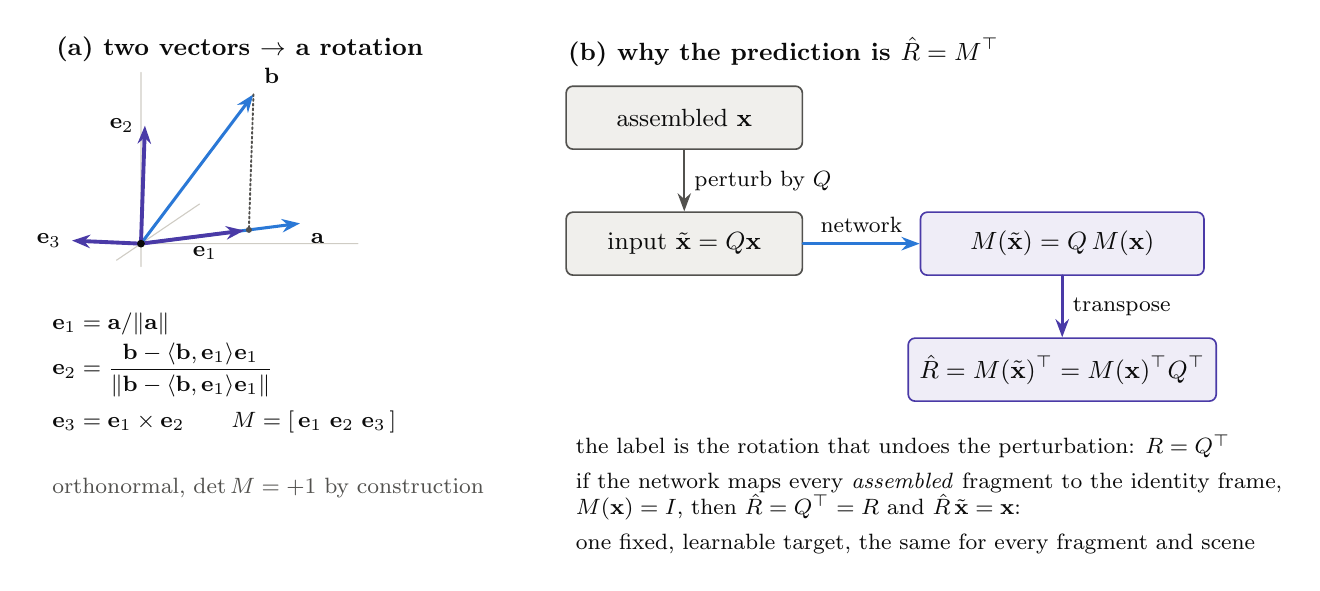
\begin{tikzpicture}
  % ---------------- (a) Gram-Schmidt ----------------
  \node[panel] at (-1.2,2.75) {(a) two vectors $\to$ a rotation};
  \begin{scope}[x={(1.45cm,0cm)}, y={(0.62cm,0.42cm)}, z={(0cm,1.45cm)}]
    \coordinate (O) at (0,0,0);
    % faint reference axes
    \draw[rule, line width=0.4pt] (-0.25,0,0) -- (1.9,0,0) (0,-0.5,0) -- (0,1.2,0) (0,0,-0.2) -- (0,0,1.5);
    % the head's two outputs
    \draw[vecarr] (O) -- (1.5,-0.25,0.25) node[below right, tlbl] {$\mathbf a$};
    \draw[vecarr] (O) -- (0.9,0.2,1.25) node[above right, tlbl] {$\mathbf b$};
    % projection of b on e1
    \draw[ink2, densely dotted, line width=0.7pt] (0.9,0.2,1.25) -- (1.018,-0.17,0.17);
    \fill[ink2] (1.018,-0.17,0.17) circle (1.1pt);
    % the frame
    \draw[outarr, line width=1.4pt] (O) -- (0.973,-0.162,0.162) node[pos=0.62, below, tlbl] {$\mathbf e_1$};
    \draw[outarr, line width=1.4pt] (O) -- (-0.103,0.322,0.941) node[left, tlbl] {$\mathbf e_2$};
    \draw[outarr, line width=1.4pt] (O) -- (-0.205,-0.933,0.297) node[left, tlbl] {$\mathbf e_3$};
    \fill[ink] (O) circle (1.4pt);
  \end{scope}
  \node[lbl, anchor=north west, align=left, text=ink] at (-1.25,-0.75) {
    $\mathbf e_1=\mathbf a/\lVert\mathbf a\rVert$\\[2pt]
    $\mathbf e_2=\dfrac{\mathbf b-\langle\mathbf b,\mathbf e_1\rangle\mathbf e_1}{\lVert\mathbf b-\langle\mathbf b,\mathbf e_1\rangle\mathbf e_1\rVert}$\\[4pt]
    $\mathbf e_3=\mathbf e_1\times\mathbf e_2$\qquad $M=[\,\mathbf e_1\ \mathbf e_2\ \mathbf e_3\,]$};
  \node[lbl, anchor=north west, align=left] at (-1.25,-2.85) {orthonormal, $\det M=+1$ by construction};

  % ---------------- (b) the convention ----------------
  \begin{scope}[shift={(5.6,0)}]
    \node[panel] at (-0.3,2.75) {(b) why the prediction is $\hat R=M^{\top}$};
    \node[box, font=\small, minimum width=3.0cm] (x) at (1.3,1.6) {assembled $\mathbf x$};
    \node[box, font=\small, minimum width=3.0cm] (xt) at (1.3,0.0) {input $\tilde{\mathbf x}=Q\mathbf x$};
    \node[outbox, font=\small, minimum width=3.6cm] (M) at (6.1,0.0) {$M(\tilde{\mathbf x})=Q\,M(\mathbf x)$};
    \node[outbox, font=\small, minimum width=3.6cm] (R) at (6.1,-1.6) {$\hat R=M(\tilde{\mathbf x})^{\top}=M(\mathbf x)^{\top}Q^{\top}$};
    \draw[arr] (x) -- node[right, tlbl] {perturb by $Q$} (xt);
    \draw[vecarr] (xt) -- node[above, tlbl] {network} (M);
    \draw[outarr] (M) -- node[right, tlbl] {transpose} (R);
    \node[lbl, anchor=north west, align=left, text=ink] at (-0.2,-2.3) {
      the label is the rotation that undoes the perturbation: $R=Q^{\top}$\\[3pt]
      if the network maps every \emph{assembled} fragment to the identity frame,\\
      $M(\mathbf x)=I$, then $\hat R=Q^{\top}=R$ and $\hat R\,\tilde{\mathbf x}=\mathbf x$:\\[3pt]
      one fixed, learnable target, the same for every fragment and scene};
  \end{scope}
\end{tikzpicture}
\end{document}
